\chapter{Supplementary Tables}
\label{app:tables}

\begin{table}[h]
\centering
\caption{The stateless control by market category at 15 minutes, on the validation
samples of the 15-minute run (balanced accuracy inside the category; $p_{\mathrm{move}}$ is
the share of samples whose mid moved within the horizon, $p_{\mathrm{up}}$ the share of
\textsc{up} among the moves).  The stateful model is the two-pass run without trees.}
\label{tab:app:cat15}
\small
\begin{fittable}\begin{tabular}{lrrccccc}
\toprule
Category & samples & markets & $p_{\mathrm{move}}$ & $p_{\mathrm{up}}$ & MR & LightGBM & stateful \\
\midrule
esports       & 162{,}228   & 1{,}266 & 0.53 & 0.48 & 0.552 & \textbf{0.589} & 0.585 \\
sports        & 3{,}117{,}846 & 6{,}844 & 0.33 & 0.48 & 0.551 & \textbf{0.621} & 0.609 \\
crypto        & 292{,}527   & 1{,}160 & 0.30 & 0.47 & 0.553 & \textbf{0.623} & 0.620 \\
weather       & 200{,}158   &   696   & 0.49 & 0.45 & 0.480 & 0.556 & \textbf{0.558} \\
politics      & 3{,}764{,}416 & 4{,}502 & 0.23 & 0.46 & 0.536 & \textbf{0.622} & 0.610 \\
economy, tech & 889{,}609   & 1{,}197 & 0.30 & 0.47 & 0.520 & \textbf{0.600} & 0.596 \\
culture       & 1{,}405{,}618 &   726   & 0.44 & 0.49 & 0.501 & \textbf{0.579} & 0.578 \\
other         & 76{,}127    &   119   & 0.27 & 0.42 & 0.518 & \textbf{0.586} & 0.580 \\
\bottomrule
\end{tabular}\end{fittable}
\end{table}

\begin{table}[h]
\centering
\caption{Univariate diagnostics of the strongest features at 1 h, on the control's
validation samples: directional hit rate on the samples that moved (best of the two
orientations), and area under the ROC curve of the feature's magnitude for separating
\textsc{const} from a move.}
\label{tab:app:univariate}
\small
\begin{fittable}\begin{tabular}{lcc}
\toprule
Feature & hit rate on moves & AUC move vs \textsc{const} \\
\midrule
mid minus its one-hour mean   & 0.573 & --- \\
level-1 imbalance             & 0.557 & --- \\
microprice minus mid          & 0.555 & --- \\
on-chain taker flow (15 min)  & 0.526 & --- \\
ten-level imbalance           & 0.508 & --- \\
tensor order-flow imbalance   & 0.500--0.505 & --- \\
time since the last mid change & --- & 0.85 \\
\midrule
\multicolumn{3}{l}{\emph{At 1 min (on the samples of the 1-minute run)}} \\
level-1 imbalance             & 0.541 & --- \\
mid changes in the last hour  & --- & 0.94 \\
time since the last mid change & --- & 0.91 \\
events in the last minute     & --- & 0.89 \\
\bottomrule
\end{tabular}\end{fittable}
\end{table}

% ── Tables and a figure of the exploratory analysis (\cref{ch:exploration}), for the technical reader ──


\begin{table}[p]
\centering
\caption{Share of the three classes among the labelled validation samples of 13 March, by
horizon (samples of the stateful models: every market of every block at the block time;
1 h, 6 h and 12 h from the causal-baseline evaluation, 1 and 15 min from the short-horizon
runs).}
\label{tab:expl:classes}
\begin{fittable}\begin{tabular}{lccc}
\toprule
Horizon & \textsc{down} & \textsc{const} & \textsc{up} \\
\midrule
1 min  & 0.057 & 0.891 & 0.052 \\
15 min & 0.164 & 0.690 & 0.146 \\
1 h    & 0.236 & 0.549 & 0.215 \\
6 h    & 0.335 & 0.354 & 0.312 \\
12 h   & 0.377 & 0.275 & 0.348 \\
\bottomrule
\end{tabular}\end{fittable}
\end{table}

\begin{table}[p]
\centering
\caption{Neighbourhood purity in the maps and in the original space at 15 min: share of
the fifteen nearest neighbours with the same label, the share expected by chance
($\sum_c p_c^2$) and their ratio.  UMAP on 50{,}000 samples, t-SNE on 20{,}000.}
\label{tab:structure:purity}
\small
\begin{tabular}{lccc ccc}
\toprule
& \multicolumn{3}{c}{UMAP} & \multicolumn{3}{c}{original space} \\
\cmidrule(lr){2-4}\cmidrule(lr){5-7}
Label & same & chance & lift & same & chance & lift \\
\midrule
prediction label (3 classes) & 0.649 & 0.524 & 1.24 & 0.662 & 0.524 & 1.26 \\
market category (8)          & 0.404 & 0.273 & 1.48 & 0.462 & 0.273 & 1.69 \\
price-level bucket (3)       & 0.488 & 0.341 & 1.43 & 0.556 & 0.341 & 1.63 \\
activity quartile (4)        & 0.423 & 0.250 & 1.69 & 0.487 & 0.250 & 1.95 \\
market identity (11{,}294)   & 0.026 & 0.0003 & 104 & 0.052 & 0.0003 & 202 \\
\bottomrule
\end{tabular}
\end{table}

\begin{table}[p]
\centering
\caption{Separability of the three classes at 15 min on the validation day, balanced
accuracy on all and on deduplicated samples.  Linear models and trees are fitted on one
million training rows; kNN on the same rows and evaluated on 300{,}000 validation samples,
with the vote of the neighbours weighted by the inverse class frequency.  LightGBM is the
G5 control of \cref{ch:stateless}, uncalibrated.}
\label{tab:structure:sep15}
\small
\begin{tabular}{lcc}
\toprule
Model & all & dedup \\
\midrule
Mean Reversion-$H$                      & 0.537 & 0.525 \\
LDA, uniform priors                     & 0.561 & 0.495 \\
Logistic regression, balanced weights   & 0.568 & 0.505 \\
Decision tree, depth 3, balanced        & 0.548 & 0.549 \\
Decision tree, depth 6, balanced        & 0.571 & 0.562 \\
kNN, $k = 5$                            & 0.532 & 0.517 \\
kNN, $k = 50$                           & 0.570 & 0.551 \\
kNN, $k = 200$                          & 0.574 & 0.553 \\
kNN, $k = 1000$                         & 0.572 & 0.551 \\
kNN, $k = 50$, 20-D random projection   & 0.564 & 0.547 \\
LightGBM G5 (control)                   & 0.616 & 0.600 \\
\bottomrule
\end{tabular}
\end{table}

\begin{table}[p]
\centering
\caption{Neighbourhood purity lift (same label among the fifteen nearest neighbours over
chance) in the original space / in the UMAP, by horizon.  Only the prediction label
depends on the horizon.}
\label{tab:structure:purityh}
\small
\begin{tabular}{lccccc}
\toprule
Lift of & 1 min & 15 min & 1 h & 6 h & 12 h \\
\midrule
prediction label   & 1.06 / 1.05 & 1.26 / 1.24 & 1.39 / 1.36 & 1.45 / 1.39 & 1.42 / 1.35 \\
market category    & 1.68 / 1.48 & 1.69 / 1.48 & 1.69 / 1.48 & 1.64 / 1.41 & 1.64 / 1.41 \\
price-level bucket & 1.63 / 1.43 & 1.63 / 1.43 & 1.64 / 1.44 & 1.61 / 1.41 & 1.60 / 1.38 \\
activity quartile  & 1.90 / 1.66 & 1.95 / 1.69 & 1.95 / 1.70 & 1.95 / 1.66 & 1.96 / 1.66 \\
market identity    & 216 / 114   & 202 / 104   & 202 / 106   & 198 / 101   & 200 / 102 \\
\bottomrule
\end{tabular}
\end{table}

\begin{table}[p]
\centering
\caption{Separability by horizon: balanced accuracy on all and deduplicated samples of the
same learners as \cref{tab:structure:sep15}.  kNN with the best $k$ on 300{,}000
samples; $\Delta$ is the difference from the control on the same samples, hour-block
bootstrap 95\% interval.}
\label{tab:structure:seph}
\footnotesize
\begin{fittable}\begin{tabular}{lcccccccccc}
\toprule
& \multicolumn{2}{c}{1 min} & \multicolumn{2}{c}{15 min} & \multicolumn{2}{c}{1 h} & \multicolumn{2}{c}{6 h} & \multicolumn{2}{c}{12 h} \\
\cmidrule(lr){2-3}\cmidrule(lr){4-5}\cmidrule(lr){6-7}\cmidrule(lr){8-9}\cmidrule(lr){10-11}
Model & all & dedup & all & dedup & all & dedup & all & dedup & all & dedup \\
\midrule
Mean Reversion-$H$     & 0.536 & 0.501 & 0.537 & 0.525 & 0.531 & 0.518 & 0.507 & 0.500 & 0.507 & 0.500 \\
LDA                    & 0.462 & 0.362 & 0.561 & 0.495 & 0.563 & 0.546 & 0.541 & 0.517 & 0.539 & 0.516 \\
Logistic regression    & 0.504 & 0.376 & 0.568 & 0.505 & 0.562 & 0.525 & 0.544 & 0.518 & 0.543 & 0.519 \\
Decision tree, depth 3 & 0.558 & 0.474 & 0.548 & 0.549 & 0.534 & 0.503 & 0.513 & 0.492 & 0.499 & 0.497 \\
Decision tree, depth 6 & 0.575 & 0.479 & 0.571 & 0.562 & 0.554 & 0.535 & 0.531 & 0.512 & 0.531 & 0.523 \\
kNN, best $k$          & 0.508 & 0.400 & 0.574 & 0.553 & 0.566 & 0.549 & 0.543 & 0.528 & 0.546 & 0.533 \\
\quad best $k$ & \multicolumn{2}{c}{20} & \multicolumn{2}{c}{200} & \multicolumn{2}{c}{200} & \multicolumn{2}{c}{1000} & \multicolumn{2}{c}{1000} \\
\quad $\Delta$ vs control & \multicolumn{2}{c}{$-10.2$ [$-11.2$, $-9.5$]} & \multicolumn{2}{c}{$-4.0$ [$-4.3$, $-3.8$]} & \multicolumn{2}{c}{$-3.6$ [$-4.0$, $-3.2$]} & \multicolumn{2}{c}{$-3.0$ [$-3.3$, $-2.6$]} & \multicolumn{2}{c}{$-2.5$ [$-2.8$, $-2.2$]} \\
LightGBM G5 (control)  & 0.609 & 0.474 & 0.616 & 0.600 & 0.602 & 0.583 & 0.572 & 0.567 & 0.572 & 0.568 \\
\bottomrule
\end{tabular}\end{fittable}
\end{table}

\begin{table}[p]
\centering
\caption{Mutual information between a feature and the label, in nats, by horizon, for the
thirteen features that are among the six most informative at some horizon (bold where they
are), the two short returns for comparison, and the sum over each group.  300{,}000 validation samples, nearest-neighbour
estimator.  Label entropy 0.42, 0.83, 1.00, 1.10, 1.09 nats.}
\label{tab:structure:mih}
\small
\begin{tabular}{lccccc}
\toprule
Feature (group) & 1 min & 15 min & 1 h & 6 h & 12 h \\
\midrule
\path{moves_60m} (G3) & \textbf{0.149} & \textbf{0.221} & \textbf{0.212} & 0.135 & 0.104 \\
\path{rv_60m} (G3) & \textbf{0.142} & \textbf{0.229} & \textbf{0.225} & 0.154 & 0.122 \\
\path{since_move} (G3) & \textbf{0.123} & \textbf{0.209} & \textbf{0.211} & 0.167 & 0.153 \\
\path{range_pos_60m} (G3) & \textbf{0.132} & \textbf{0.182} & 0.171 & 0.110 & 0.090 \\
\path{mid_minus_mean60} (G3) & 0.104 & \textbf{0.187} & \textbf{0.190} & 0.127 & 0.099 \\
\path{usd_15m} (G4) & \textbf{0.112} & 0.114 & 0.099 & 0.062 & 0.055 \\
\path{ntr_15m} (G4) & \textbf{0.105} & 0.088 & 0.070 & 0.032 & 0.028 \\
\path{ret_15m} (G1) & 0.097 & 0.162 & 0.143 & 0.080 & 0.060 \\
\path{ret_1h} (G1) & 0.087 & 0.158 & 0.165 & 0.112 & 0.089 \\
\path{micro_minus_mid_ticks} (G2) & 0.044 & \textbf{0.166} & \textbf{0.270} & \textbf{0.410} & \textbf{0.457} \\
\path{imb1} (G2) & 0.041 & 0.143 & \textbf{0.233} & \textbf{0.362} & \textbf{0.408} \\
\path{log_bid_sz0} (G2) & 0.039 & 0.116 & 0.184 & \textbf{0.290} & \textbf{0.334} \\
\path{log_ask_sz0} (G2) & 0.035 & 0.100 & 0.160 & \textbf{0.261} & \textbf{0.303} \\
\path{log_bid_sz10} (G2) & 0.024 & 0.085 & 0.139 & \textbf{0.217} & \textbf{0.242} \\
\path{log_duration_h} (G5) & 0.095 & 0.148 & 0.178 & \textbf{0.223} & \textbf{0.262} \\
\midrule
sum over G1 (price) & 0.63 & 1.16 & 1.31 & 1.16 & 1.10 \\
sum over G2 (book) & 0.38 & 1.10 & 1.68 & 2.51 & 2.81 \\
sum over G3 (flow and clock) & 1.15 & 1.45 & 1.38 & 0.87 & 0.73 \\
sum over G4 (trades) & 0.60 & 0.75 & 0.76 & 0.51 & 0.46 \\
sum over G5 (static) & 0.28 & 0.37 & 0.42 & 0.45 & 0.49 \\
\bottomrule
\end{tabular}
\end{table}

\begin{figure}[p]
\centering
\resizebox{\textwidth}{!}{\begin{tikzpicture}
\begin{axis}[thesis, width=0.62\textwidth, height=5.4cm, xmode=log, log basis x=10, xlabel={$k$ (neighbours)}, ylabel={balanced accuracy, all samples}, xmin=3, xmax=1600, ymin=0.44, ymax=0.70, legend pos=outer north east, legend columns=1, legend cell align=left]
\addplot[vizA, thick, mark=*, mark size=1.6pt] coordinates {(5,0.4913) (20,0.5084) (50,0.5015) (200,0.4919) (1000,0.4692)};
\addlegendentry{kNN 1 min}
\addplot[vizB, thick, mark=square*, mark size=1.6pt] coordinates {(5,0.5324) (20,0.5597) (50,0.5702) (200,0.5743) (1000,0.5719)};
\addlegendentry{kNN 15 min}
\addplot[vizC, thick, mark=triangle*, mark size=1.6pt] coordinates {(5,0.5200) (20,0.5498) (50,0.5593) (200,0.5664) (1000,0.5646)};
\addlegendentry{kNN 1 h}
\addplot[vizD, thick, mark=diamond*, mark size=1.6pt] coordinates {(5,0.4972) (20,0.5197) (50,0.5323) (200,0.5402) (1000,0.5431)};
\addlegendentry{kNN 6 h}
\addplot[vizInk, thick, mark=pentagon*, mark size=1.6pt] coordinates {(5,0.5023) (20,0.5272) (50,0.5370) (200,0.5460) (1000,0.5460)};
\addlegendentry{kNN 12 h}
\end{axis}
\end{tikzpicture}
}
\caption{Balanced accuracy of the balanced-vote kNN against $k$ at every horizon, on
300{,}000 validation samples.  The optimum moves from $k = 20$ at 1 min to $k = 1000$ at
6 and 12 h.}
\label{fig:structure:knn}
\end{figure}

\begin{table}[t]
\centering
\caption{What every layout of the market map keeps (\cref{sec:expl:graph:weight}).  For
every market the fifteen nearest markets on the page are compared with its fifteen nearest
markets in the 64-dimensional trading space (fidelity), with its category, with its
contract template (\cref{sec:expl:templates}) and, for the five- and fifteen-minute crypto
contracts, with its first trading day.  Islands are the groups of at least 150 markets
found by HDBSCAN on the page, and the noise share is the share of markets in no island.}
\label{tab:graph:mapmetrics}
\small
\begin{fittable}\begin{tabular}{lrrrrrr}
\toprule
layout & fidelity & same category & same template & same day & islands & noise \\
 & (\%) & (\%) & (\%) & (\%) & & (\%) \\
\midrule
similarity only ($w = 0$) & 20.4 & 76.0 & 49.0 & 25.4 & 129 & 21.2 \\
category block, $w = 0.25$ & 19.3 & 96.1 & 57.4 & 24.8 & 95 & 11.1 \\
category block, $w = 0.5$ & 18.3 & 99.7 & 59.3 & 24.0 & 39 & 4.8 \\
category block, $w = 0.75$ & 18.3 & 99.9 & 59.3 & 24.3 & 34 & 4.8 \\
category block, $w = 1$ & 18.4 & 100.0 & 59.6 & 24.5 & 58 & 9.4 \\
supervised, target weight 0 & 20.1 & 85.3 & 53.5 & 24.8 & 109 & 16.4 \\
supervised, target weight 0.5 & 19.9 & 96.2 & 57.9 & 24.5 & 84 & 10.7 \\
50 neighbours, $w = 0$ & 15.8 & 75.3 & 47.7 & 23.2 & 72 & 14.8 \\
contract-template block, weight 0.5 & 15.6 & 95.8 & 98.1 & 24.9 & 97 & 4.7 \\
first-day axis, weight 0.5 & 13.9 & 75.7 & 48.4 & 71.5 & 148 & 28.4 \\
\bottomrule
\end{tabular}\end{fittable}
\end{table}

\begin{figure}[p]
\centering
\begin{subfigure}{0.86\textwidth}
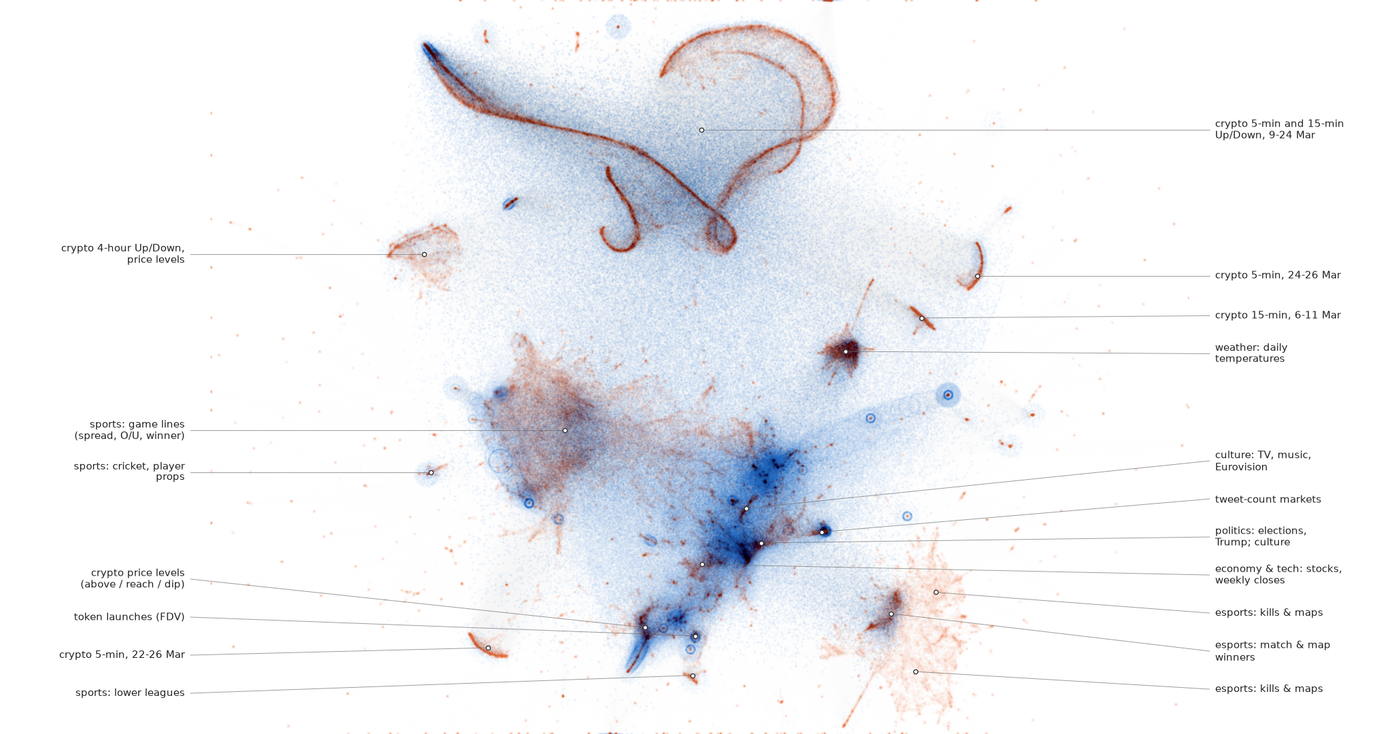
\includegraphics[width=\textwidth]{figures/graph/graph_map_w025.png}
\caption{Category block, $w = 0.25$.}
\end{subfigure}

\medskip
\begin{subfigure}{0.86\textwidth}
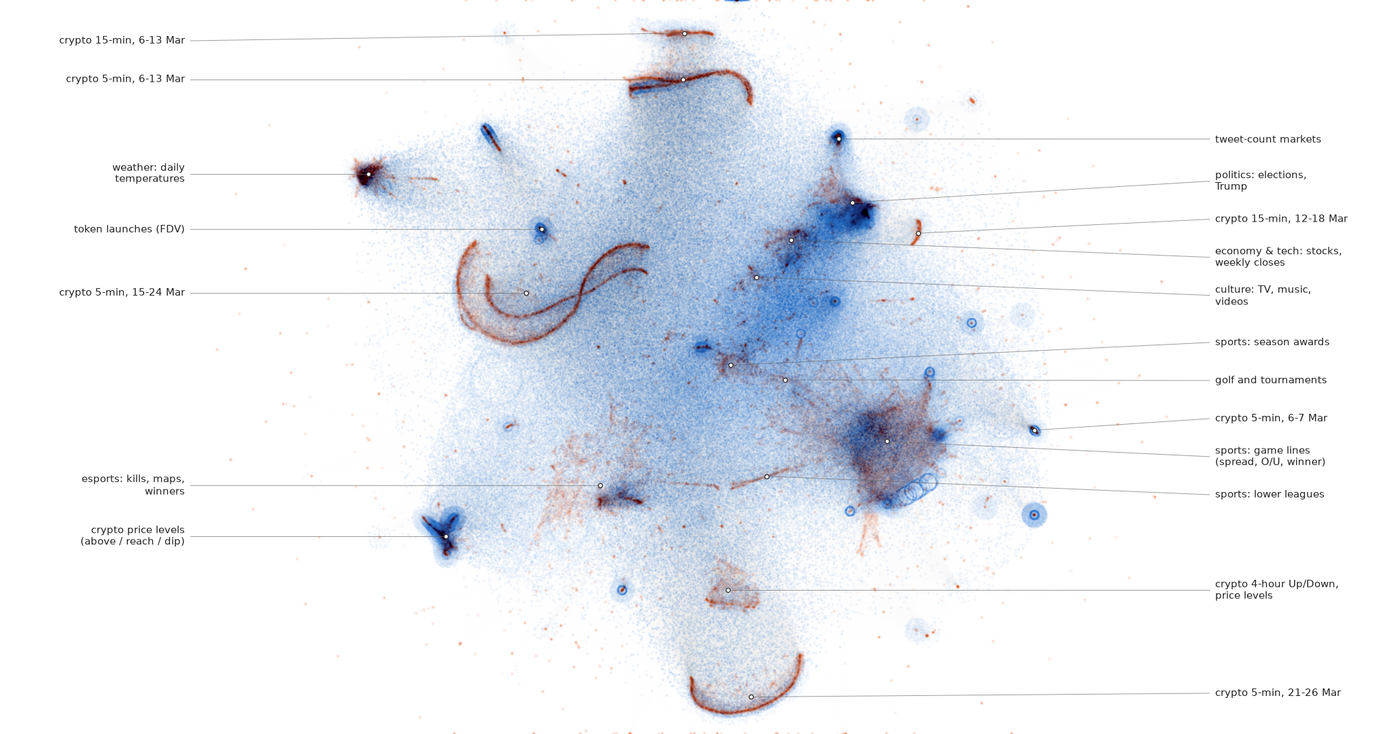
\includegraphics[width=\textwidth]{figures/graph/graph_map_supervised.png}
\caption{Supervised layout, target weight 0.5.}
\end{subfigure}
\caption{The market map at the other positions of the dial of \cref{sec:expl:graph:weight},
with the largest islands labelled as in \cref{fig:graph:maps} (wallets in blue, markets in
orange).  (a) At $w = 0.25$ the five- and fifteen-minute crypto contracts form one ribbon
ordered by date at the top, sports and esports regions of their own, and politics, culture
and economy still touch at the centre.  (b) The supervised layout keeps the islands of
\cref{fig:graph:map:sim}, the short crypto contracts one island per period of days, and
gathers the categories into regions.  (c), (d) At $w = 0.75$ and $w = 1$ every category is
a continent, and the two maps differ only in how compact the continents are.}
\label{fig:graph:othermaps}
\end{figure}

\begin{figure}[p]
\ContinuedFloat
\centering
\begin{subfigure}{0.86\textwidth}
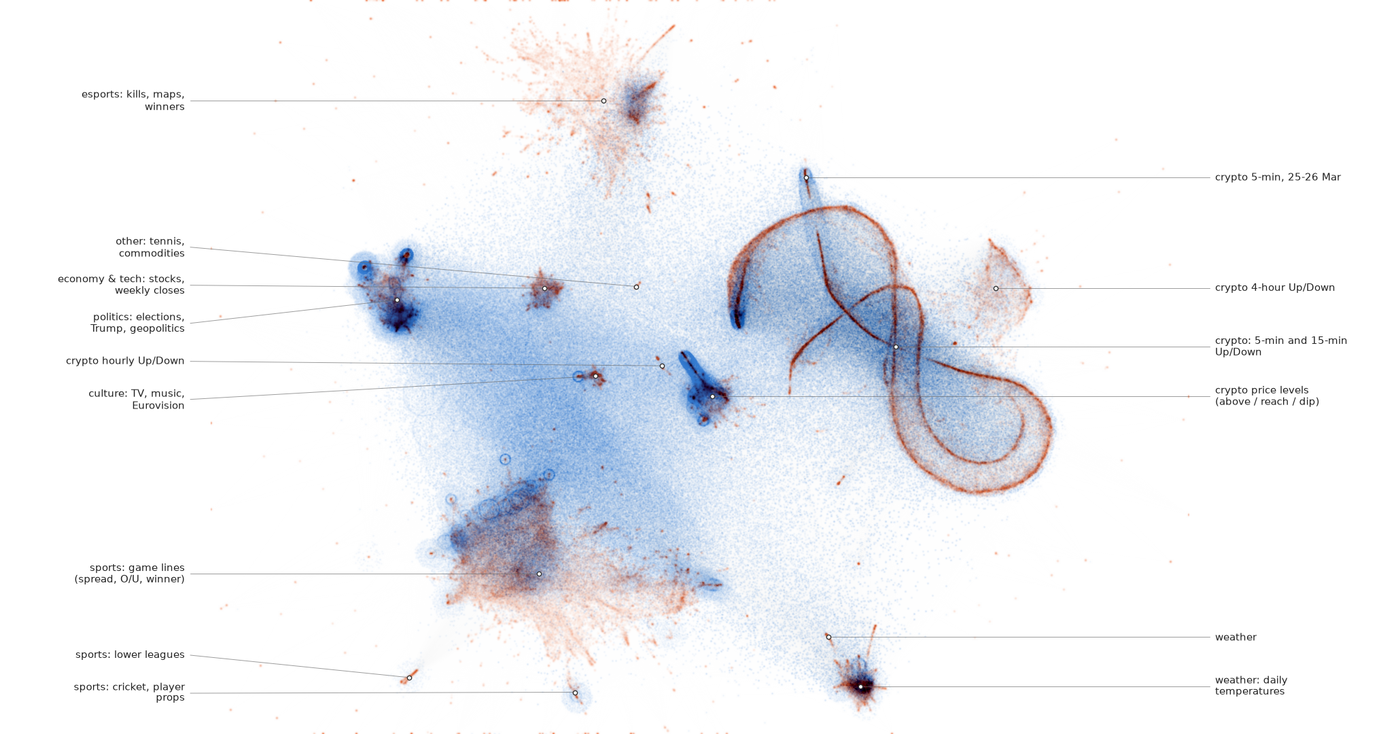
\includegraphics[width=\textwidth]{figures/graph/graph_map_w075.png}
\caption{Category block, $w = 0.75$.}
\end{subfigure}

\medskip
\begin{subfigure}{0.86\textwidth}
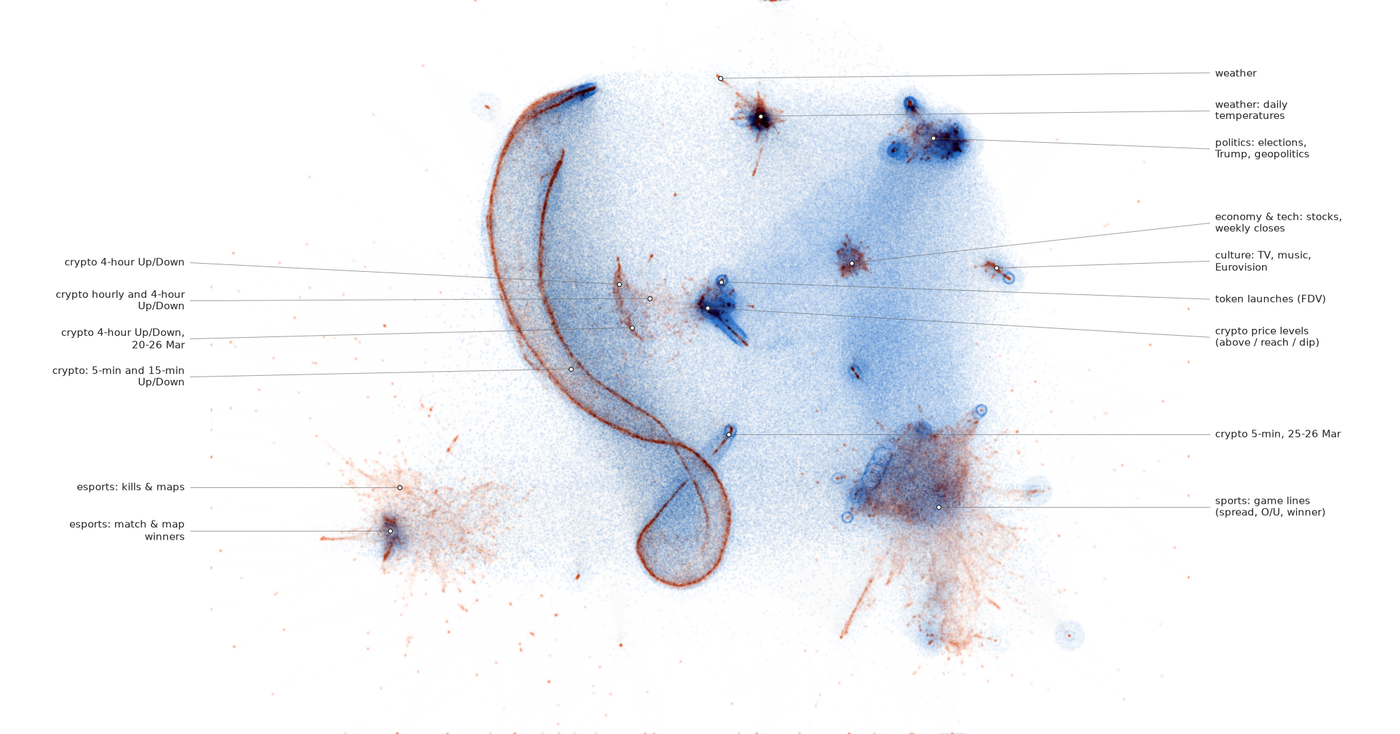
\includegraphics[width=\textwidth]{figures/graph/graph_map_w100.png}
\caption{Category block, $w = 1$.}
\end{subfigure}
\caption{(continued)}
\end{figure}

\begin{figure}[p]
\centering
\begin{subfigure}{0.32\textwidth}
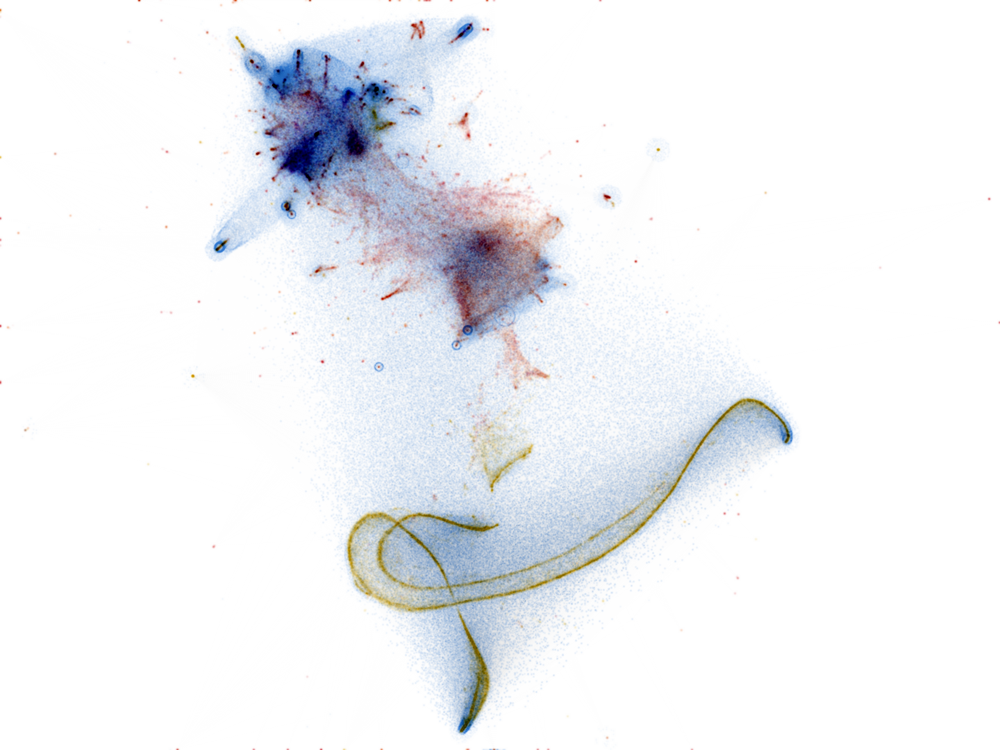
\includegraphics[width=\textwidth]{figures/graph/graph_map_nn50.png}
\caption{50 neighbours, $w = 0$.}
\end{subfigure}\hfill
\begin{subfigure}{0.32\textwidth}
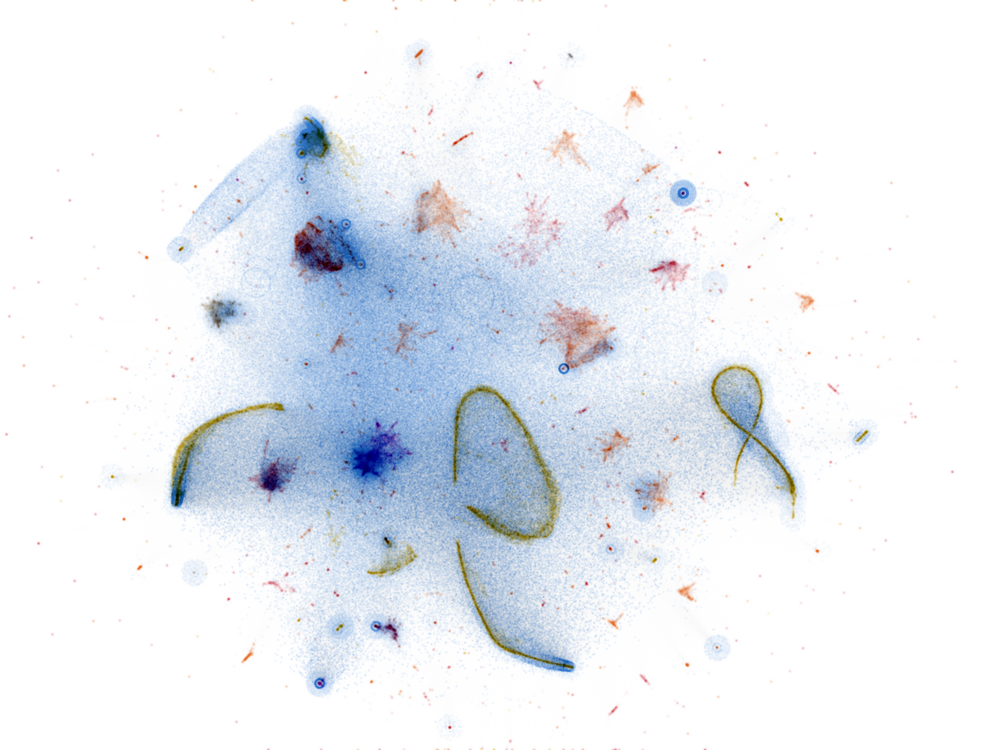
\includegraphics[width=\textwidth]{figures/graph/graph_map_template.png}
\caption{Contract-template block.}
\end{subfigure}\hfill
\begin{subfigure}{0.32\textwidth}
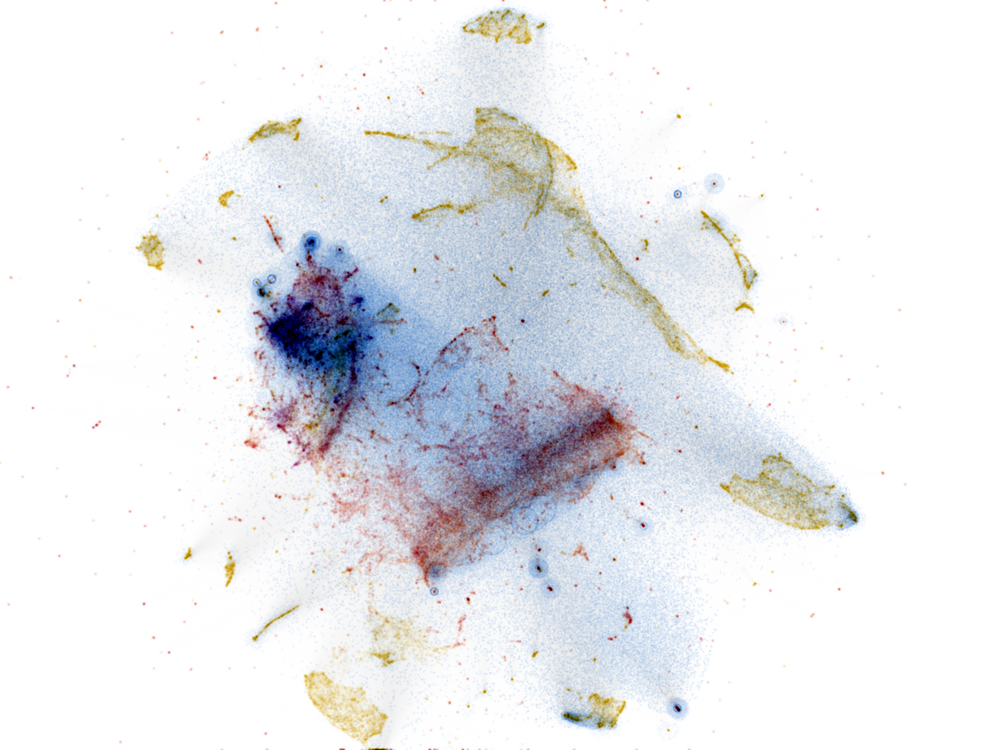
\includegraphics[width=\textwidth]{figures/graph/graph_map_day.png}
\caption{First-day axis.}
\end{subfigure}
\caption{Three other layouts of the market map, markets coloured by category as in
\cref{fig:graph:weights}.  (a) With fifty neighbours instead of fifteen the per-day islands
of the short crypto contracts chain into one ribbon, and sports, politics and esports share
one region.  (b) A block of indicator coordinates of the contract template
(\cref{sec:expl:templates}) in place of the category, with weight 0.5, gives a catalogue of
contract types: 98\% of the page neighbours of a market share its template, in many small
islands that cut across the categories.  (c) The first trading day of the market as an
extra coordinate, with weight 0.5, makes the date the first partition: 72\% of the page
neighbours of a short crypto contract are contracts of the same day, three times the share
of the other layouts, and every category is sliced by date.}
\label{fig:graph:extramaps}
\end{figure}
